\chapter{面向Real2Sim的仿真动态混合隐式场}
最近的隐式神经渲染方法已经证明,通过预测仅由一组 RGB 图像监督的体积密度和颜色,可以为复杂场景学习准确的新视图合成。然而,现有方法仅限于学习将所有场景对象编码到单个神经网络中的静态场景的有效表示,并且缺乏表示动态场景和分解为单个场景对象的能力。本文提出了一种将动态场景分解为场景图的神经渲染方法。我们提出了一种学习的场景图表示,对场景中物体对象的刚体变换和场景内容(外观和几何等)分别进行编码,以高效地在新视角下和全新的物体信息(如轨迹信息、外观信息)下进行真实感的渲染。在此基础之上,本文对每一类具有共同特征的物体(如所有车辆、摩托)学习共同类别隐式表征,并为每个物体学习单独隐式编码,来加速网络的收敛性能。

\section{简介}

从一组图像中进行视图合成和场景重建是计算机图形学和计算机视觉中的基本问题。研究人员投入了大量精力来增强计算机通过复制视觉内容来创建图片的能力。这为电影制作、机器人模拟、增强现实和电话会议等许多行业带来了巨大的价值。计算机图形学通过首先创建一个虚拟 3D 世界然后模仿光在世界中的传输方式以产生逼真的场景渲染来使用物理学对图像生成过程进行建模。为了产生视觉上吸引人的结果,基于物理的渲染需要大量的计算资源、昂贵的手动资产创建和物理建模。现有实时渲染引擎生成的图像仍然存在显着的真实感差距,降低了它们对机器人模拟和训练数据增强的影响。数据驱动的图像编辑方法,如图像合成等在过去几年中受到了极大的关注。他们专注于通过从大规模视觉数据训练的生成模型来加强渲染图像真实感。然而,大多数工作并不对应于底层逼真的 3D 世界,因此,生成的 2D 内容不能直接用于自动驾驶Real2Sim2Real应用。

近年来,随着隐式场方\cite{mildenhall_nerf_2020, barron_mip-nerf_2022, muller_instant_2022}的快速发展,在静态场景中进行高质量渲染已经日趋成熟,然而现有方法通常使用一个单一的场景表示网络来建模整个场景,因此只能建模单一静态场景,而无法建模场景中的动态物体。虽然有部分方法使用基于不确定性的可优化的隐式编码的方法忽略场景中的动态信息\cite{martin-brualla_nerf_2021},但是这类方法无法对动态物体进行渲染,更不用说面向Real2Sim的自动驾驶仿真。

本文提出一个用于表示复杂动态场景的隐式场景建模方法。通过将一个动态自动驾驶场景分解为背景节点和一组物体节点的有向图,分别对每个节点学习一个单独的隐式表征,本文可以实现对动态复杂场景的高质量建模,并且可以对物体运行轨迹和外观进行简单的编辑。

\begin{figure}[ht]
    \centering
    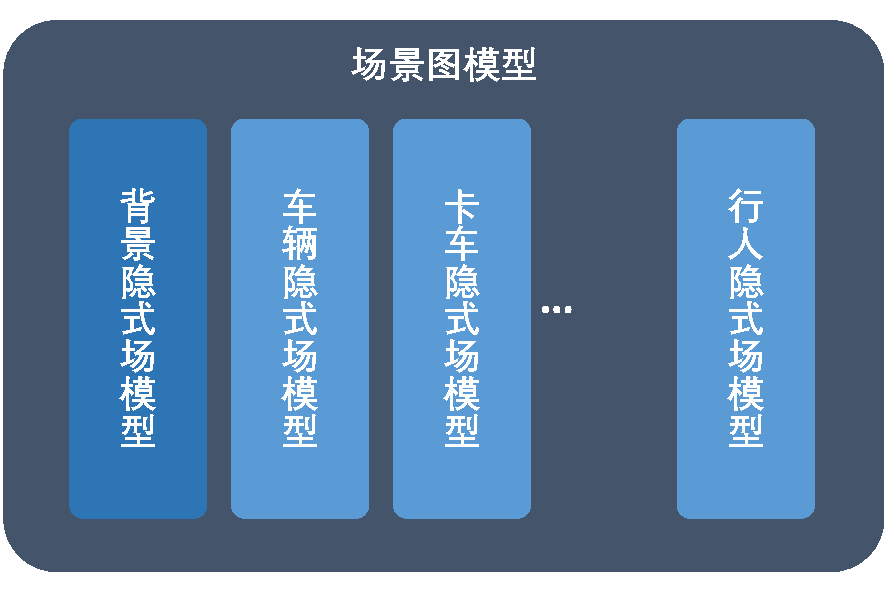
\includegraphics[width=0.6\textwidth]{undergraduate-thesis/images/scene-graph.pdf}
    \caption{场景图模型}
    \label{fig:scene-graph model}
\end{figure}

\section{场景图建模}

本节将介绍使用混合隐式场景图模型对复杂动态场景进行建模的方法。 在本文中,我们将场景图定义为一个五元组\cite{ost_neural_2021}:
\begin{equation}
    \mathcal{S} = <W, C, F, L, E>,
\end{equation}
其中,$W$为根节点,$C$为一组相机,其中主要存储相机的内参数信息,$F$为叶子节点的集合,包含背景隐式模型节点和所有物体模型节点,$L$是每类物体的可学习隐式编码,与$F$中的物体类别一一对应,$F$中的场景模型均基于本文在第\ref{chapter: omninerf}章所提出的混合隐式场景表示,$E$为在每帧中从物体节点到其对应相机节点的刚体转换矩阵,对于每个物体的三维边界框,我们用三维世界系下坐标$\mathbf{p}_o = [x, y, z]$、边界框大小尺度$s_o = [s_x, s_y, s_z]$和旋转向量$r = [r_{row}, r_{yaw}, r_{pitch}]$表示。

\begin{figure}[ht]
    \centering
    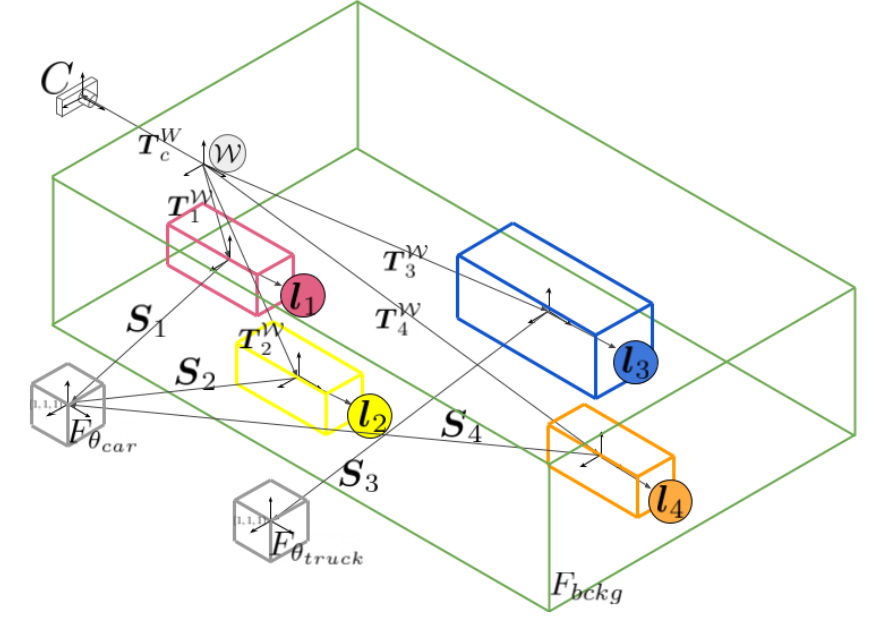
\includegraphics[width=0.8\textwidth]{undergraduate-thesis/images/nsg-scene-graph visualization.png}
    \caption{NSG\cite{ost_neural_2021}中提出的场景图分解方法。}
    \label{fig:NSG scene graph}
\end{figure}

\newcommand{\bgweight}{{\theta_{bckg}}}
\newcommand{\bgmodel}{F_{\bgweight}}
\newcommand{\classweight}{{\theta_{c}}}
\newcommand{\classmodel}{F_{\classweight}}
\newcommand{\xbf}{{\mathbf{x}}}
\newcommand{\dbf}{{\mathbf{d}}}
\newcommand{\cbf}{{\mathbf{c}}}
\newcommand{\po}{{\mathbf{p}_o}}
\newcommand{\latent}{{\mathbf{l}_o}}
\newcommand{\xo}{{\xbf_o}}
\newcommand{\dobj}{{\dbf_o}}
\newcommand{\xw}{{\xbf_w}}
\newcommand{\objpose}{\mathbf{T}_o^w}
\newcommand{\campose}{\mathbf{T}_c^w}
\newcommand{\ray}{{\mathbf{r}}}
\newcommand{\tobj}{{t_{o}}}
\newcommand{\tino}{{t_{o, in}}}
\newcommand{\touto}{{t_{o, out}}}
\newcommand{\tinw}{{t_{w, in}}}
\newcommand{\toutw}{{t_{w, out}}}

\subsection{背景节点}
对于背景建模,我们简单地直接使用此前提出的混合隐式表达作为场景模型。该模型$\bgmodel: (\xbf, \dbf) \to (\cbf, \sigma)$
将采样点的世界坐标$\xbf$和观察角度$\dbf$隐式映射到辐射颜色$\cbf$和体密度$\sigma$。

\subsection{动态物体节点}
对于动态物体,我们对第\ref{chapter: omninerf}章中的混合隐式场进行增补以使用同一个物体类别模型在同类物体中不同实例间泛化。对于每个物体,本文从其局部归一化空间中进行采样得到局部空间中的坐标$\po$,并对每个物体学习其单独的隐式编码$\latent$。因此,物体的隐式函数表达可以写作:
\begin{equation}
[\cbf(\xo), \sigma(\xo)] = \classmodel(\latent, \po, \xo, \dobj).
\end{equation}

\subsubsection{隐式物体编码学习}
为动态场景中的每个对象训练单独的场景表示很容易导致大量模型和训练工作。相反,本文的目标是最小化表示场景中所有对象的模型数量,通过学习一个类别隐式模型和若干物体隐式编码,并在渲染时将隐式编码$\latent$和物体局部坐标同时输入物体隐式表征网络,即可以达到类似使用每个物体单独网络的效果,即:
\begin{equation}
    F_{\theta_o}(\xo, \dobj) = \classmodel(\xo, \dobj, \latent).
\end{equation}

\section{组合渲染}
当物体在场景中移动时,物体边界框的世界坐标$\po$也自然会随之移动,因此我们在进行渲染的时候也需要将物体模型渲染的辐射量进行相应的移动。设物体中的一个采样点在世界系下的坐标为$\xw$,通过物体位姿的转换可以得到其在该物体的局部边界框坐标系下的坐标$\xo$:
\begin{equation}
    \xo = s_o\objpose\xw,
\end{equation}
其中$\xo\in[-1,1]$,$\objpose$是从世界坐标系到物体坐标系的位置变换。

当给定物体位姿$\{\objpose\}$和对应相机位姿时,便可以使用场景图模型进行新视角渲染。对于任意给定的一个针孔相机$C$,其内参数矩阵$K$和外参数$\campose$,可以发射一组$H\times W$的射线簇,其中每条射线可以表示为$\ray = \mathbf{o} + t\dbf$。本文在每条射线上使用基于Proposal网络的采样策略得到$N$个采样点。

为了将每个采样点分配到所应使用的模型上,本文计算射线$\ray$和物体边界框的交点。对于每条和物体边界框相较的射线, 必然存在两个采样点,这里将其进入点和射出点在世界系和物体局部坐标系下的射线深度分别写作$(\tinw, \toutw), (\tino, \touto)$。

在获得射线与物体边界框的交点后,可以将所有射线深度在这一区间中的采样点$X_o =\{\xo |\tino \leq t_{o} \leq \touto\}$分配到对应渲染模型中进行推理,其余点使用背景模型进行推理。
当所有采样点的辐射和体密度值均已求得后,可以使用体渲染方法将采样点序列渲染为输出RGB颜色。

\section{场景图编辑}

当对一个动态场景获得其训练好的场景图后,便可以对其中的动态物体进行编辑。本文在这里介绍对车辆行驶轨迹和外观进行编辑的方法。

\subsection{车辆行驶轨迹编辑}
对于场景图$\mathcal{S}$中的叶子节点$F_i$,其轨迹可以表示为时间到边界框位姿的函数:
\begin{equation}
    f_{traj}: \quad t\to<\po, s_o, r_o>.
\end{equation}

为了修改行驶轨迹,只需对位姿函数进行相应编辑,如若要使车辆在空间上按向量$\Delta\po$平移,则可生成新的轨迹为:
\begin{equation}
    f_{traj}^{trans}(t) = <\po + \Delta\po, s_o, r_o>
\end{equation}

同理,也可以对车辆进行旋转、缩放:
\begin{align}
    f_{traj}^{scale}(t) &= <\po, s_o * s', r_o>\\
    f_{traj}^{rot}(t) &= <\po, s_o, r_o + \Delta r_o>
\end{align}

通过组合上述操作,即可对车辆的行驶轨迹进行编辑。编辑效果请见实验章节。

\subsection{车辆外观编辑}
前文提到,本文对一类具有共同特征的物体使用相同的隐式表征网络,因此该网络可以在同类物体的不同实例间泛化,对于每个特定物体,只需提供一个隐式编码向量即可生成对应的物体级别网络。因此如果希望对物体形状、外观进行编辑,可以通过编辑隐式编码来实现。

对于类别网络$\classmodel$和物体隐式编码$\latent$表示的物体,若需要对该物体进行修改,一种可行的办法是在该编码上添加高斯噪声$\varepsilon\sim\mathcal{N}(0, 1)$:
\begin{equation}
    \latent' := \latent + \varepsilon
\end{equation}

这种方法可以有效改变物体外观、形状属性,但是由于高斯噪声的随机性,很难对编辑后的物体结果提前预知。为了对编辑进行控制,可以在两个同类物体的隐式编码间进行插值:
\begin{equation}
    \latent' := p\latent^{(0)} + (1 - p)\latent^{(1)}, \quad p\in[0,1]
\end{equation}

随着扩散模型\cite{ho_denoising_2020, poole_dreamfusion_2022, yang_learning_2023}的发展,通过添加和定向去除高斯噪声实现基于文本指令导向的编辑也成为可能。由于该主题与本文Real2Sim仿真场景重建的主线不符,本文不再讨论相关话题。

\section{本章小结}  
本章提出了一个基于场景图的动态复杂场景重建方法。使用视频和带标注的输入数据,我们的方法学习了多个动态和静态场景元素的连续隐式场景表示,将场景分解为多个独立的节点。我们通过使用学习的图结构在场景中生成新的对象排列来验证学习的场景图方法。这种方法还大大提高了神经渲染管道的效率,这对于从视频序列中学习至关重要。

由于该场景图分解方法是一个通用框架,而对于每个节点,其内在场景表示实现可以随意更换,因而场景图方法的迭代更新可以依靠场景表示的技术发展而实现。场景图方法目前存在的限制,如无法准确表示人体的复杂骨骼、非刚体运动等也均可以通过定制具体类别的场景表示实现。因此在未来,一个重要的发展方向是对场景图中不同类别的物体分别使用类别专属的网络结构,以适应该类物体的天然特性。

除此以外,目前的场景图方法依赖于手工的数据标注,而单目目标检测方法通常具有尺度、平移偏差,从而无法在多视角三维重建场景中被有效利用。因此一个可预见的未来发展方向是将目标检测融入场景表示中,使用端到端的场景图构建方法从只有传感器数据的数据集中学习混合隐式场景图。